\section{Identité du site}

Cette section fait office de charte d'identité / charte graphique de notre plateforme.

\subsection{VroomMates}

Nous avons choisi "VroomMates" afin de représenter la plateforme. Il s'agit d'un jeu de mots avec le mot "roommates", l'idée est de rappeler le principe de collocation et en quelques-sorte l'appliquer dans le monde du covoiturage.

\subsection{Logo}

\begin{figure}[th]
\centering

\includegraphics[width=\linewidth]{medias/logos.png}
\decoRule
\caption{Différents logos de la plateforme}
\end{figure}

En ce qui concerne le logo, celui-ci est l'une des premières choses que nous avons faite au sein du groupe. Nous pensons que la réalisation d'un logo constitue en outre la base de notre charte graphique: toute l'identité visuelle y allait être forcément influencée. 
L'identité du site (voir \ref{Identité du site}) ainsi que le choix des couleurs (voir \ref{Palette de couleurs}) s'est, de ce fait, décidé ici même.
Nous avons aussi fait le choix de faire une version raccourcie, que nous allons utiliser en tant qu'image de profil sur la plateforme ou de favicon pour le client.

\subsection{Identité du site}
\label{Identité du site}


Nous voulons avoir un certain lien de proximité avec l'utilisateur et renvoyer une certaine image de jeunesse que l'on pourrait retrouver dans certaines start-ups connues;
Pour adopter ce style décontracté / jovial, nous avons décidé d'employer une police d'écriture arrondie et sans éperons, \href{https://fonts.google.com/specimen/Baloo+2}{Baloo 2} est ainsi un candidat idéal.

\subsection{Palette de couleurs}
\label{Palette de couleurs}

\begin{figure}[th]
\centering
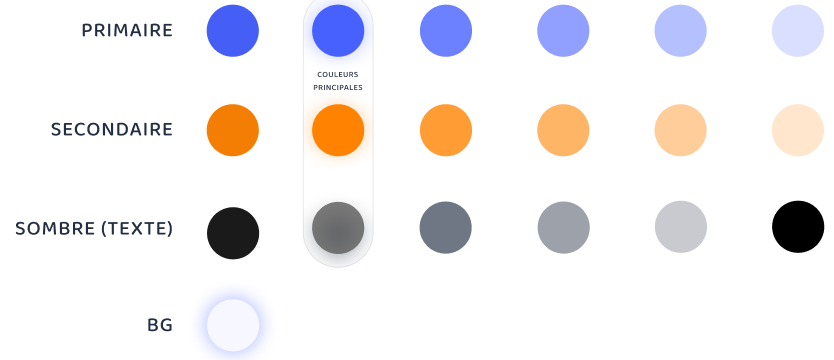
\includegraphics[width=\linewidth]{medias/palette.png}
\decoRule
\caption{Palette de couleur}
\end{figure}

En guise de palette de couleur, nous nous sommes inspirés de la dualité entre l'orange et le bleu, présents sur le site de Metz Numeric School. Ces deux couleurs opposées sont la base de la quasi-totalité de notre site, et nous avons créé plusieurs variantes de ces deux couleurs (sous formes de dégradés).
